\documentclass{article}

\usepackage{fancyhdr}
\usepackage{extramarks}
\usepackage{amsmath}
\usepackage{amsthm}
\usepackage{amsfonts}
\usepackage{tikz}
\usepackage[plain]{algorithm}
\usepackage{algpseudocode}
\usepackage{enumerate}
\usepackage{amssymb}
\usepackage{adjustbox}
\usepackage{multirow}
\usepackage{graphicx}
\usepackage{afterpage}
\usepackage{subcaption}


\usetikzlibrary{automata,positioning}

%
% Basic Document Settings
%

\topmargin=-0.45in
\evensidemargin=0in
\oddsidemargin=0in
\textwidth=6.5in
\textheight=9.0in
\headsep=0.25in

\linespread{1.1}

\pagestyle{fancy}
\lhead{\hmwkAuthorName}
\chead{\hmwkClass\ (\hmwkClassInstructor\ \hmwkClassTime): \hmwkTitle}
\rhead{\firstxmark}
\lfoot{\lastxmark}
\cfoot{\thepage}

\renewcommand\headrulewidth{0.4pt}
\renewcommand\footrulewidth{0.4pt}

\setlength\parindent{0pt}

%
% Create Problem Sections
%

\newcommand{\enterProblemHeader}[1]{
    \nobreak\extramarks{}{Problem \arabic{#1} continued on next page\ldots}\nobreak{}
    \nobreak\extramarks{Problem \arabic{#1} (continued)}{Problem \arabic{#1} continued on next page\ldots}\nobreak{}
}

\newcommand{\exitProblemHeader}[1]{
    \nobreak\extramarks{Problem \arabic{#1} (continued)}{Problem \arabic{#1} continued on next page\ldots}\nobreak{}
    \stepcounter{#1}
    \nobreak\extramarks{Problem \arabic{#1}}{}\nobreak{}
}

\setcounter{secnumdepth}{0}
\newcounter{partCounter}
\newcounter{homeworkProblemCounter}
\setcounter{homeworkProblemCounter}{1}
\nobreak\extramarks{Problem \arabic{homeworkProblemCounter}}{}\nobreak{}

%
% Homework Problem Environment
%
% This environment takes an optional argument. When given, it will adjust the
% problem counter. This is useful for when the problems given for your
% assignment aren't sequential. See the last 3 problems of this template for an
% example.
%
\newenvironment{homeworkProblem}[1][-1]{
    \ifnum#1>0
        \setcounter{homeworkProblemCounter}{#1}
    \fi
    \section{Problem \arabic{homeworkProblemCounter}}
    \setcounter{partCounter}{1}
    \enterProblemHeader{homeworkProblemCounter}
}{
    \exitProblemHeader{homeworkProblemCounter}
}

%
% Homework Details
%   - Title
%   - Due date
%   - Class
%   - Section/Time
%   - Instructor
%   - Author
%

\newcommand{\hmwkTitle}{Tutorial 10}
\newcommand{\hmwkDueDate}{March 30, 2021}
\newcommand{\hmwkClass}{CZ2003}
\newcommand{\hmwkClassTime}{SS3}
\newcommand{\hmwkClassInstructor}{Assoc Prof Alexei Sourin}
\newcommand{\hmwkAuthorName}{\textbf{Pang Yu Shao}}
\newcommand{\hmwkAuthorID}{\textbf{U1721680D}}

%
% Title Page
%

\title{
    \vspace{2in}
    \textmd{\textbf{\hmwkClass:\ \hmwkTitle}}\\
    \normalsize\vspace{0.1in}\small{Due\ on\ \hmwkDueDate\ at 10:30am}\\
    \vspace{0.1in}\large{\textit{\hmwkClassInstructor\ - \hmwkClassTime}}
    \vspace{3in}\\
    \hmwkAuthorName\\
    \hmwkAuthorID
}

\date{29/03/2021}

\renewcommand{\part}[1]{\textbf{\large Part \Alph{partCounter}}\stepcounter{partCounter}\\}

%
% Various Helper Commands
%

% Useful for algorithms
\newcommand{\alg}[1]{\textsc{\bfseries \footnotesize #1}}

% For derivatives
\newcommand{\deriv}[1]{\frac{\mathrm{d}}{\mathrm{d}x} (#1)}

% For partial derivatives
\newcommand{\pderiv}[2]{\frac{\partial}{\partial #1} (#2)}

% Integral dx
\newcommand{\dx}{\mathrm{d}x}

% Alias for the Solution section header
\newcommand{\solution}{\textbf{\large Solution}}

% Probability commands: Expectation, Variance, Covariance, Bias
\newcommand{\E}{\mathrm{E}}
\newcommand{\Var}{\mathrm{Var}}
\newcommand{\Cov}{\mathrm{Cov}}
\newcommand{\Bias}{\mathrm{Bias}}

\begin{document}

\maketitle

\pagebreak

\begin{homeworkProblem}
   Propose an animation model in implicit representation, which defines the movement of a unit sphere
   along a 3D helical curve in a uniform speed along the z-direction (see Figure Q1). The helical curve
   has radius 30, period 10, and 15 full rotations, as shown below. The animation sequence should have
   100 frames. \\
   \begin{figure}[H]
      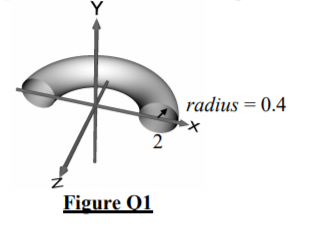
\includegraphics[width=8cm]{fig/q1.PNG}
      \centering
   \end{figure}
   \textbf{Solution}\\\\
   Unit Sphere centered at $(x_c, y_c, z_y)$: $f(x,y,z) = 1 - (x-x_c)^2 - (y-y_c)^2 - (z-z_c)^2$

   Step 1: Represent the path by parametric equations:\\
   $x_c(\tau) = 30cos(30\pi\tau)$\\
   $y_c(\tau) = 30sin(30\pi\tau)$\\
   $z_c(\tau) = 15*10*\tau = 150\tau$\\\\

   Step 2: Link path to object, represent object with parametric/implicit function:\\
   $f(x,y,z,\tau) = 1 - (x-x_c(\tau))^2 - (y-y_c(\tau))^2 - (z-z_c(\tau))^2$\\\\

   Step 3: Control speed of animation (uniform speed) by defining $\tau = f(k)$:\\
   $\tau = f(k) = \frac{k-1}{100-1}$\\\\
   $x_c(k) = 30cos(30\pi\frac{k-1}{100-1})$\\
   $y_c(k) = 30sin(30\pi\frac{k-1}{100-1})$\\
   $z_c(k) = 150\frac{k-1}{100-1}$\\\\
   $f(x,y,z,k) = 1 - (x-x_c(k))^2 - (y-y_c(k))^2 - (z-z_c(k))^2$\\\\
   $f(x,y,z,k) = 1 - (x-30cos(30\pi\frac{k-1}{100-1}))^2 - (y-30sin(30\pi\frac{k-1}{100-1}))^2 - (z-150\frac{k-1}{100-1})^2$\\\\

   where k is the frame index, $1\leq k \leq 100$

   

\end{homeworkProblem}
\pagebreak
\begin{homeworkProblem}
   With reference to Figure Q2, propose parametric functions defining animated transformation of the
   2D polygon labelled as “A” into the 2D disk labelled as “B”. The animation takes 256 frames and
   involves deceleration. 
   \begin{figure}[H]
      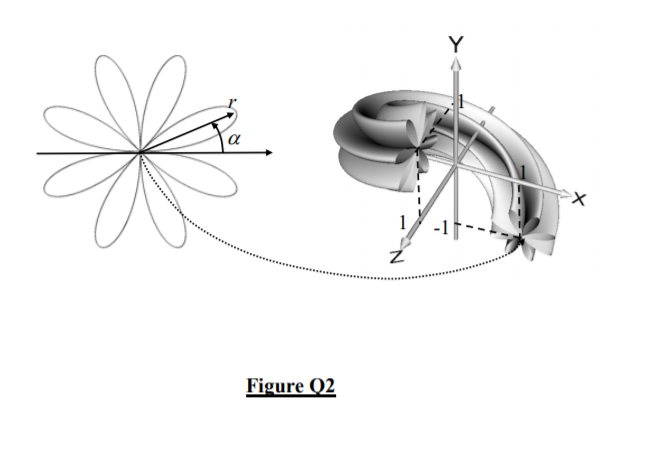
\includegraphics[width=8cm]{fig/q2.PNG}
      \centering
   \end{figure}
   \textbf{Solution}\\
   First, define A and B parametrically:\\
   $x_A(u,v) = 1 + 3u$\\
   $y_A(u,v) = 1 + 2v$\\
   $u,v \in [0,1]$\\\\
   $x_B(u,v) = 7+2vcos(2\pi u)$\\
   $y_B(u,v) = 2+2vsin(2\pi u)$\\
   $u,v \in [0,1]$\\\\
  
   Next, add animation:\\
   $x(u,v,\tau) = (1-\tau)x_A(u,v) + \tau x_B(u,v)$\\
   $y(u,v,\tau) = (1-\tau)y_A(u,v) + \tau y_B(u,v)$\\
   $u,v,\tau \in [0,1]$\\\\

   Lastly, control speed of animation by defining $\tau$ (deccelerating):\\
   $\tau = f(k) = sin(\frac{\pi}{2}\frac{k-1}{256-1})$\\
   Therefore,\\
   $x(u,v,k) = (1-sin(\frac{\pi}{2}\frac{k-1}{256-1}))(1+3u) + sin(\frac{\pi}{2}\frac{k-1}{256-1})(7+2vcos(2\pi u))$\\
   $y(u,v,k) = (1-sin(\frac{\pi}{2}\frac{k-1}{256-1}))(1+2v) + sin(\frac{\pi}{2}\frac{k-1}{256-1})(2+2vsin(2\pi u))$\\
   $u,v \in [0,1]$, where k is the frame index, $1\leq k \leq 256$
   \begin{figure}[H]
      \begin{subfigure}{.33\textwidth}
        \centering
        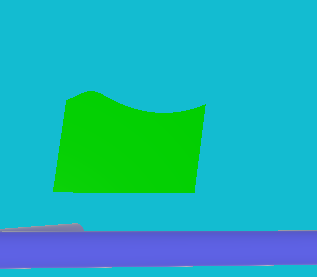
\includegraphics[width=.8\linewidth]{fig/q2a}
      \end{subfigure}%
      \begin{subfigure}{.33\textwidth}
        \centering
        
\includegraphics[width=.8\linewidth]{fig/q2b}
      \end{subfigure}
      \begin{subfigure}{.33\textwidth}
         \centering
         
\includegraphics[width=.8\linewidth]{fig/q2c}
        \end{subfigure}
   \end{figure}
\end{homeworkProblem}

\pagebreak
\begin{homeworkProblem}
   Propose a mathematical model that implements morphing which transforms a solid unit 
   sphere centered at the origin into a solid cylinder parallel to the Z-axis, center at the 
   point (1,1,3) and height of 6. The morphing sequence has 200 frames and involves acceleration. 
   The frame index starts at 1\\\\
   
   \textbf{Solution}\\
   Let A be the solid sphere and B be the solid cylinder\\
   First, define A and B parametrically:\\
   $x_A(u,v,w) = wcos(2\pi u)cos(\pi v)$\\
   $y_A(u,v,w) = wcos(2\pi u)sin(\pi v)$\\
   $z_A(u,v,w) = wsin(2\pi u)$\\
   $u,v,w \in [0,1]$\\\\
   (Assuming radius of cylinder is 1)\\
   $x_B(u,v,w) = 1+vcos(2\pi u)$\\
   $y_B(u,v,w) = 1+vsin(2\pi u)$\\
   $z_B(u,v,w) = 6w$\\
   $u,v,w \in [0,1]$\\\\
  
   Next, add animation:\\
   $x(u,v,w,\tau) = (1-\tau)x_A(u,v,w) + \tau x_B(u,v,w)$\\
   $y(u,v,w,\tau) = (1-\tau)y_A(u,v,w) + \tau y_B(u,v,w)$\\
   $z(u,v,w,\tau) = (1-\tau)z_A(u,v,w) + \tau z_B(u,v,w)$\\
   $u,v,w,\tau \in [0,1]$\\\\

   Lastly, control speed of animation by defining $\tau$ (accelerating):\\
   $\tau = f(k) = 1 - cos(\frac{\pi}{2}\frac{k-1}{200-1})$\\\\

   Therefore,\\
   $x(u,v,w,k) = (1-(1 - cos(\frac{\pi}{2}\frac{k-1}{200-1})))(wcos(2\pi u)cos(\pi v)) + (1 - cos(\frac{\pi}{2}\frac{k-1}{200-1}))(1+vcos(2\pi u))$\\
   $y(u,v,w,k) = (1-(1 - cos(\frac{\pi}{2}\frac{k-1}{200-1})))(wcos(2\pi u)sin(\pi v)) + (1 - cos(\frac{\pi}{2}\frac{k-1}{200-1}))(1+vsin(2\pi u))$\\
   $z(u,v,w,k) = (1-(1 - cos(\frac{\pi}{2}\frac{k-1}{200-1})))(wsin(2\pi u)) + (1 - cos(\frac{\pi}{2}\frac{k-1}{200-1}))(6w))$\\
   $u,v,w \in [0,1]$, where k is the frame index, $1\leq k \leq 200$\\\\

   \begin{figure}[H]
      \begin{subfigure}{.33\textwidth}
        \centering
        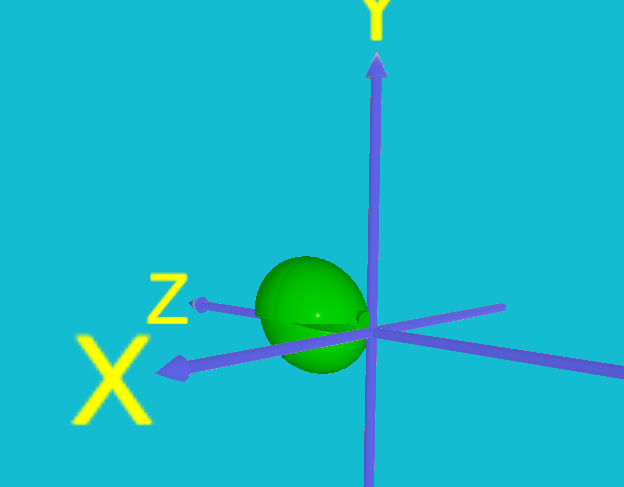
\includegraphics[width=.8\linewidth]{fig/q3a}
      \end{subfigure}%
      \begin{subfigure}{.33\textwidth}
        \centering
        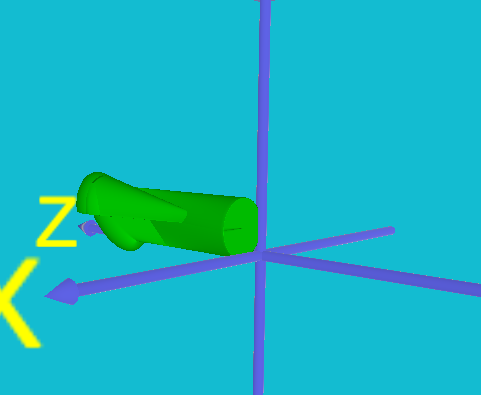
\includegraphics[width=.8\linewidth]{fig/q3b}
      \end{subfigure}
      \begin{subfigure}{.33\textwidth}
         \centering
         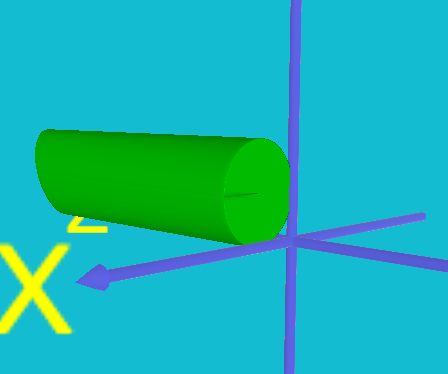
\includegraphics[width=.8\linewidth]{fig/q3c}
        \end{subfigure}
   \end{figure}
\end{homeworkProblem}

\end{document}